% Options for packages loaded elsewhere
\PassOptionsToPackage{unicode}{hyperref}
\PassOptionsToPackage{hyphens}{url}
\documentclass[
]{article}
\usepackage{xcolor}
\usepackage{amsmath,amssymb}
\setcounter{secnumdepth}{-\maxdimen} % remove section numbering
\usepackage{iftex}
\ifPDFTeX
  \usepackage[T1]{fontenc}
  \usepackage[utf8]{inputenc}
  \usepackage{textcomp} % provide euro and other symbols
\else % if luatex or xetex
  \usepackage{unicode-math} % this also loads fontspec
  \defaultfontfeatures{Scale=MatchLowercase}
  \defaultfontfeatures[\rmfamily]{Ligatures=TeX,Scale=1}
\fi
\usepackage{lmodern}
\ifPDFTeX\else
  % xetex/luatex font selection
\fi
% Use upquote if available, for straight quotes in verbatim environments
\IfFileExists{upquote.sty}{\usepackage{upquote}}{}
\IfFileExists{microtype.sty}{% use microtype if available
  \usepackage[]{microtype}
  \UseMicrotypeSet[protrusion]{basicmath} % disable protrusion for tt fonts
}{}
\makeatletter
\@ifundefined{KOMAClassName}{% if non-KOMA class
  \IfFileExists{parskip.sty}{%
    \usepackage{parskip}
  }{% else
    \setlength{\parindent}{0pt}
    \setlength{\parskip}{6pt plus 2pt minus 1pt}}
}{% if KOMA class
  \KOMAoptions{parskip=half}}
\makeatother
\usepackage{longtable,booktabs,array}
\newcounter{none} % for unnumbered tables
\usepackage{calc} % for calculating minipage widths
% Correct order of tables after \paragraph or \subparagraph
\usepackage{etoolbox}
\makeatletter
\patchcmd\longtable{\par}{\if@noskipsec\mbox{}\fi\par}{}{}
\makeatother
% Allow footnotes in longtable head/foot
\IfFileExists{footnotehyper.sty}{\usepackage{footnotehyper}}{\usepackage{footnote}}
\makesavenoteenv{longtable}
\usepackage{graphicx}
\makeatletter
\newsavebox\pandoc@box
\newcommand*\pandocbounded[1]{% scales image to fit in text height/width
  \sbox\pandoc@box{#1}%
  \Gscale@div\@tempa{\textheight}{\dimexpr\ht\pandoc@box+\dp\pandoc@box\relax}%
  \Gscale@div\@tempb{\linewidth}{\wd\pandoc@box}%
  \ifdim\@tempb\p@<\@tempa\p@\let\@tempa\@tempb\fi% select the smaller of both
  \ifdim\@tempa\p@<\p@\scalebox{\@tempa}{\usebox\pandoc@box}%
  \else\usebox{\pandoc@box}%
  \fi%
}
% Set default figure placement to htbp
\def\fps@figure{htbp}
\makeatother
\setlength{\emergencystretch}{3em} % prevent overfull lines
\providecommand{\tightlist}{%
  \setlength{\itemsep}{0pt}\setlength{\parskip}{0pt}}
\usepackage{bookmark}
\IfFileExists{xurl.sty}{\usepackage{xurl}}{} % add URL line breaks if available
\urlstyle{same}
\hypersetup{
  hidelinks,
  pdfcreator={LaTeX via pandoc}}

\author{}
\date{}

\begin{document}

\section{AIRE-Trace: A Standardized Prospective Evaluation Protocol for
Online Agent-Failure
Warning}\label{aire-trace-a-standardized-prospective-evaluation-protocol-for-online-agent-failure-warning}

\begin{center}\rule{0.5\linewidth}{0.5pt}\end{center}

\textbf{{[}AUTHOR 1 NAME{]}} {[}AUTHOR 1 DEPARTMENT{]} {[}AUTHOR 1
INSTITUTION{]} {[}CITY, COUNTRY{]} {[}AUTHOR 1 EMAIL{]}

\textbf{{[}AUTHOR 2 NAME{]}} (if applicable) {[}AUTHOR 2 DEPARTMENT{]}
{[}AUTHOR 2 INSTITUTION{]} {[}CITY, COUNTRY{]} {[}AUTHOR 2 EMAIL{]}

\emph{Submitted to: {[}IEEE CONFERENCE NAME --- TO BE SELECTED{]}}
\emph{Submission Date: {[}SUBMISSION DATE --- TO BE DETERMINED{]}}

\begin{center}\rule{0.5\linewidth}{0.5pt}\end{center}

\subsection{Abstract}\label{abstract}

The increasing deployment of autonomous agentic systems creates demand
for mechanisms that provide prospective warning of task failure from
partial execution trajectories, rather than retrospectively diagnosing
failure after it occurs. Prior work on online agent-failure warning
(including PrefixGuard, AgentForesight, and Trajectory Guard) has
demonstrated that prefix-based failure prediction is a viable research
direction, but these methods each use their own datasets, prefix
definitions, calibration procedures, and metrics. Consequently,
comparative claims across method families are difficult to interpret.

This paper presents AIRE-Trace: a standardized, prospective, prefix-only
evaluation protocol for online agent-failure warning that fixes
information visibility, failure-target definition, alert semantics,
calibration procedure, false-alarm constraints, lead-time measurement,
and compute accounting. The protocol is applied to representative
heuristic (H1--H4), classical machine-learning (M1), and sequence-model
(S1, S2) warning methods on the TerminalBench trajectory corpus.

The study population consists of 636 reconstructed episodes -- 19.18\%
of 3,316 declared source rows -- split task-disjointly into TRAIN (163
episodes), CALIBRATION (57 episodes), and TEST (416 episodes). Of 317
failed TEST episodes, 257 carried usable failure-onset annotations
sufficient for prospective evaluation. Across seven evaluated models at
checkpoint horizon K=30, Mode A (TerminalBench) AUROC ranged from 0.5074
to 0.6371. S1 (Random Forest) achieved the highest observed AUROC
(0.6371, 95\% CI {[}0.5885, 0.6745{]}). Under a 5\% false-alarm rate
(FAR) constraint, prospective Recall@FAR was near zero across all
evaluated models. Paired episode-cluster bootstrap testing (B=1,000,
Holm--Bonferroni correction) showed S1 had statistically significant
AUROC advantages over S2, H2, and H3, but not over M1, H1, or H4. For
AUPRC, S1's advantage was statistically significant only against S2.
Feature ablation identified that removing error and retry signals
(feat\_tool\_error\_count and feat\_retry\_count) produced the largest
observed discrimination degradation (Delta\_AUROC = -0.1069). The
overall Pairwise Direction Consistency (PDC) across 21 informative pairs
was 0.8294 (coverage 0.881). These findings indicate that available
trajectory-prefix structural features contain limited prospective
failure information under strict operational false-alarm constraints,
and that comparative rankings are partially but not universally stable
across metrics.

\textbf{Index Terms:} Agentic systems, failure warning, prospective
evaluation, trajectory analysis, standardized benchmarking, online
monitoring, calibration, bootstrap inference.

\begin{center}\rule{0.5\linewidth}{0.5pt}\end{center}

\subsection{I. Introduction}\label{i.-introduction}

\subsubsection{A. Motivation}\label{a.-motivation}

The widespread deployment of autonomous agentic systems has raised new
reliability questions that standard outcome benchmarking cannot fully
answer. Benchmarks such as AgentBench {[}1{]}, AgentBoard {[}2{]}, and
GAIA {[}3{]} measure whether an agent ultimately succeeds or fails on a
task. This final-outcome evaluation is necessary but insufficient for
monitoring purposes: by the time the outcome is observed, the agent has
already consumed resources and potentially caused unrecoverable side
effects.

Prospective failure warning addresses a different and complementary
question: given only the portion of the trajectory observed so far (a
prefix), can a monitor produce a timely alert that the episode will
likely fail before the outcome is known? This early-warning capability
would enable intervention -- pausing the agent, escalating to human
review, or switching strategies -- before failure becomes irreversible.

\subsubsection{B. Prior Work and the Comparative
Gap}\label{b.-prior-work-and-the-comparative-gap}

Recent work has shown that prefix-based failure prediction is
achievable. PrefixGuard {[}7{]} achieves AUPRC of 0.900 on WebArena and
0.557 on TerminalBench under its own evaluation protocol, demonstrating
that prefix-based monitoring is feasible across multiple benchmarks.
Direct numerical comparison with AIRE-Trace results is not appropriate
due to differences in prefix representation, feature regime, and
calibration protocol. AgentForesight {[}8{]} employs a
reinforcement-learning-trained 7B online auditor for risk estimation.
Trajectory Guard {[}9{]} applies real-time sequence anomaly detection to
agent trajectories. These methods collectively establish that
prospective warning from partial trajectories is a viable line of
research with documented discriminative capability.

However, these methods each use their own datasets, prefix definitions,
calibration procedures, evaluation metrics, and operating points. No
existing work cross-compares heuristic, classical machine-learning, and
sequence-model warning methods under one fixed protocol. Consequently,
it is unclear whether reported comparative advantages between method
families in individual papers are robust to a common evaluation
protocol, or are partially artifacts of differing evaluation conditions.

\subsubsection{C. AIRE-Trace
Contribution}\label{c.-aire-trace-contribution}

AIRE-Trace does not propose a new detector architecture and does not
claim that prospective warning itself is novel. Instead, it addresses a
different methodological question: given that prospective warning is
achievable in principle, how should comparative warning capability be
evaluated when methods must operate under a fixed, deployment-relevant
false-alarm budget?

The specific contribution is a standardized, prospective, prefix-only
evaluation protocol for online agent-failure warning -- fixing
information visibility (pre-onset prefix only), failure-target
definition, alert semantics, calibration procedure, false-alarm
constraints, lead-time measurement, and compute accounting -- applied to
representative warning methods under a common harness.

The conceptual boundary distinguishing this work from adjacent
approaches: - Attribution approaches (e.g., AgentRx {[}5{]}, Who\&When
Pro {[}6{]}) ask: where or why did this already-failed run go wrong?
They are retrospective and require the full trajectory. - Warning
approaches (e.g., PrefixGuard, AgentForesight) ask: what is the
probability of eventual failure, given only the prefix, while the
outcome remains unknown? They are prospective. - AIRE-Trace asks: do
comparative performance claims for warning methods remain consistent
when those methods are evaluated under identical constraints? It is an
evaluation-protocol contribution, not a new warning method.

\subsubsection{D. Research Question}\label{d.-research-question}

\begin{quote}
Do comparative performance claims for online agent-failure warning
methods remain consistent when different methods are evaluated under
identical information, target, alert, calibration, lead-time, and
compute constraints?
\end{quote}

\subsubsection{E. Experimental Scope}\label{e.-experimental-scope}

The evaluation uses 636 reconstructed episodes split task-disjointly
into TRAIN (163), CALIBRATION (57), and TEST (416). Seven baseline
methods are evaluated in Mode A using trajectory prefixes up to K=30
steps.

\subsubsection{F. Main Empirical
Findings}\label{f.-main-empirical-findings}

\begin{itemize}
\tightlist
\item
  Mode A AUROC ranged from 0.5074 (H3) to 0.6371 (S1).
\item
  S1 achieved the highest observed AUROC but was not universally
  statistically superior.
\item
  Under 5\% FAR constraint, prospective Recall@FAR was near zero across
  all models.
\item
  Error and retry signals showed the strongest association with
  discrimination capability (Delta\_AUROC = -0.1069 at A4 ablation).
\item
  PDC = 0.8294 (coverage = 0.881) indicates partially consistent but not
  universally stable rankings.
\end{itemize}

\subsubsection{G. Contributions Summary}\label{g.-contributions-summary}

\begin{enumerate}
\def\labelenumi{\arabic{enumi}.}
\tightlist
\item
  A standardized, auditable, prospective evaluation protocol for online
  agent-failure warning enforcing FAR \textless= 5\%, episode-level
  evaluation semantics, and onset-boundary enforcement.
\item
  An empirical comparison of seven representative warning methods under
  the common protocol on a reconstructed trajectory corpus.
\item
  A Gate 6 operational analysis distinguishing prospective early-warning
  recall from post-onset late-detection activity.
\item
  A component-level feature ablation study (A0--A6) identifying the
  association between structural trace signals and discrimination
  performance.
\item
  A Pairwise Direction Consistency (PDC) analysis of metric-ranking
  stability.
\item
  Transparent reporting of provenance-repair limitations and population
  coverage constraints.
\end{enumerate}

\begin{center}\rule{0.5\linewidth}{0.5pt}\end{center}

\subsection{II. Related Work}\label{ii.-related-work}

\subsubsection{A. Agent Outcome
Benchmarking}\label{a.-agent-outcome-benchmarking}

Outcome benchmarks {[}1{]}{[}2{]}{[}3{]} establish performance baselines
for agent capabilities but do not provide mechanisms for prospective
mid-execution monitoring. TRAIL {[}4{]} articulates the need for robust
evaluation methods for agentic workflow traces, introduces a formal
taxonomy of error types, and presents 148 human-annotated traces for
trace-debugging evaluation.

\subsubsection{B. Retrospective Failure
Attribution}\label{b.-retrospective-failure-attribution}

Post-hoc failure attribution methods identify where or why a trajectory
went wrong after failure has occurred. AgentRx {[}5{]} provides post-hoc
localization of critical failure steps. Who\&When Pro {[}6{]} addresses
retrospective attribution using 12,326 trajectories with controlled
failure injection. By construction, these approaches require the
complete trajectory and ground-truth failure state and cannot produce
warnings during execution. AgentProcessBench {[}11{]} introduces
step-level quality evaluation using 1,000 trajectories and 8,509
human-labeled step annotations (ternary: correct/neutral/erroneous).
These step-quality labels require the complete trajectory with known
outcome and are retrospective by construction.

\subsubsection{C. Prospective Agent-Failure
Warning}\label{c.-prospective-agent-failure-warning}

PrefixGuard {[}7{]} demonstrates prefix-based warning monitors,
achieving AUPRC of 0.900 on WebArena and 0.557 on TerminalBench under
its own evaluation protocol with typed-step adapters. Direct numerical
comparison with AIRE-Trace results is not appropriate due to differences
in prefix representation, feature regime, and calibration protocol; both
studies use TerminalBench, but under distinct evaluation conditions.
AgentForesight {[}8{]} employs an RL-trained 7B-parameter auditor.
Trajectory Guard {[}9{]} applies real-time sequence anomaly detection.

These works establish prospective prefix-based warning as a viable
research direction, but each operates in isolation. No existing work
cross-compares heuristic, classical-ML, sequence-model, and LLM-monitor
warning methods under one fixed protocol. Advani {[}10{]} characterizes
false success in LLM agents across 9,876 tau2-Bench and 1,879 AppWorld
trajectories, showing that lightweight TF-IDF detectors achieve AUROC
0.83-0.95 for false-success detection while LLM judges fail to exceed
AUROC 0.65 on tau2-Bench. This work addresses task-completion monitoring
rather than mid-trajectory prospective warning.

\subsubsection{D. Evaluation Methodology for Sequential
Predictions}\label{d.-evaluation-methodology-for-sequential-predictions}

Prefix-level predictions exhibit within-episode dependence because
prefixes from the same episode share the outcome label. Episode-cluster
bootstrapping is the appropriate procedure when the observational unit
is the episode rather than the individual prefix. Cameron, Gelbach, and
Miller {[}12{]} establish the pairs cluster bootstrap as the appropriate
inference procedure when observations are dependent within clusters;
resampling entire clusters (episodes in our case) rather than individual
observations (prefixes) preserves the within-cluster correlation
structure. Holm {[}13{]} introduced the sequentially rejective multiple
test procedure for step-down control of the familywise error rate
without requiring independence among tests.

\begin{center}\rule{0.5\linewidth}{0.5pt}\end{center}

\subsection{III. Problem Formulation}\label{iii.-problem-formulation}

\subsubsection{A. Agent Trajectory and
Episode}\label{a.-agent-trajectory-and-episode}

An agent episode consists of a sequence of events e1, e2, \ldots, eT
produced by an autonomous agent executing a task. Each event contains
role information (agent, tool, user, system), action type (message, tool
call, tool result), tool names, error indicators, and other structural
metadata. The episode has an eventual outcome: eventual\_success or
eventual\_failure.

\subsubsection{B. Failure Onset}\label{b.-failure-onset}

For TerminalBench episodes:

\begin{verbatim}
t_onset = min(incorrect_step_ids)
\end{verbatim}

If this field is absent or empty, the episode is onset-unannotated and
excluded from onset-dependent prospective metrics (Recall@FAR, lead
time) while remaining eligible for ranking metrics (AUROC, AUPRC, Brier,
ECE).

\subsubsection{C. Prefix and Checkpoint}\label{c.-prefix-and-checkpoint}

At checkpoint t in \{1, \ldots, min(Ti, K)\}, a monitor accesses only
the prefix (e1, \ldots, et). The checkpoint schedule is
outcome-independent and episode-symmetric.

An alert at checkpoint t is valid (prospective) if and only if t
\textless= t\_onset. An alert at t \textgreater{} t\_onset is a late
detection; it does not constitute actionable early warning. These
prospective evaluation semantics are visualized in Fig. 3.

\begin{figure}
\centering
\pandocbounded{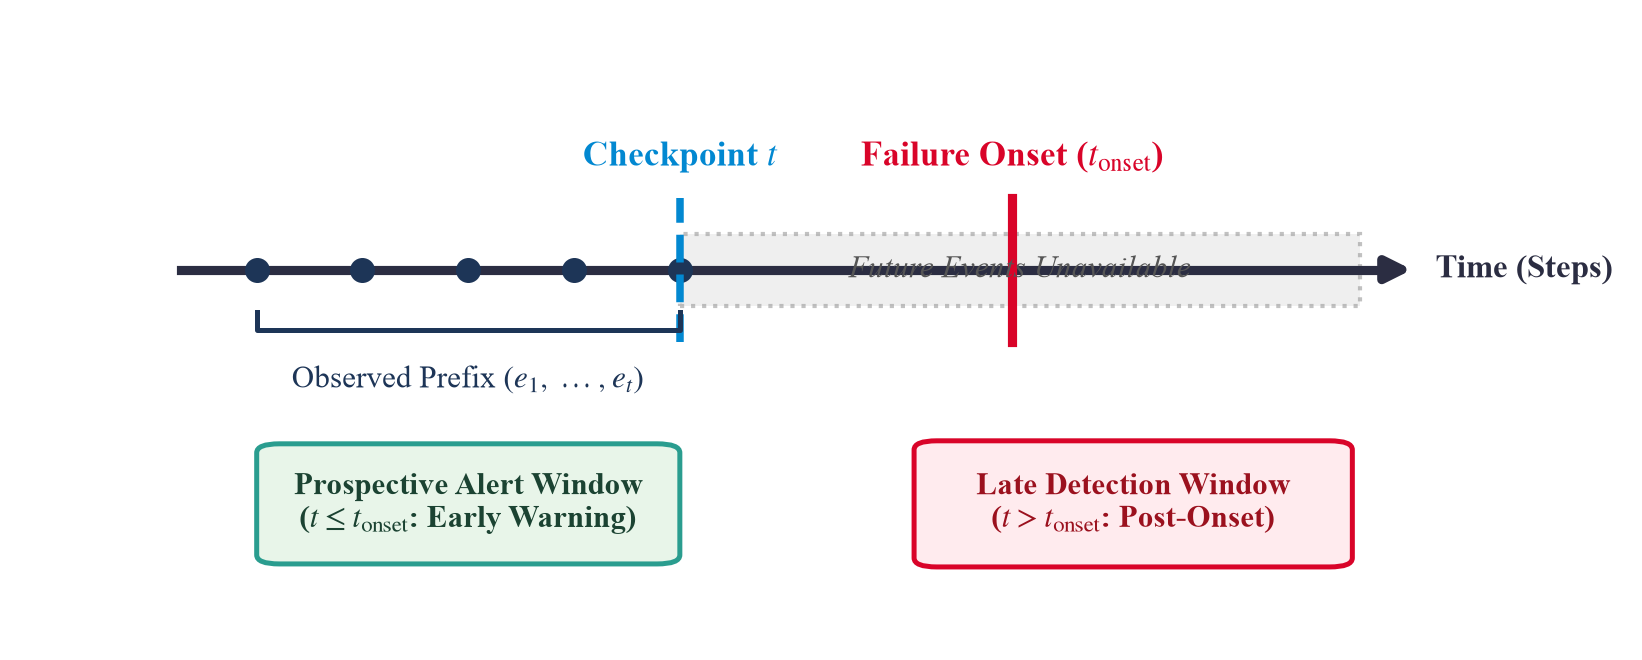
\includegraphics[keepaspectratio,alt={Fig. 3. Prospective prefix evaluation semantics. At each permitted checkpoint, the monitor observes only the trajectory information available up to that point. Alerts at or before the annotated failure onset are prospective detections; alerts after onset are analyzed separately as late detections.}]{figures/ieee/fig3_prospective_prefix.png}}
\caption{Fig. 3. Prospective prefix evaluation semantics. At each
permitted checkpoint, the monitor observes only the trajectory
information available up to that point. Alerts at or before the
annotated failure onset are prospective detections; alerts after onset
are analyzed separately as late detections.}
\end{figure}

Late detections are reported separately in the operational analysis
(Section IX) and excluded from Recall@FAR.

The conceptual flow of the overall architecture is illustrated in Fig.
1.

\begin{figure}
\centering
\pandocbounded{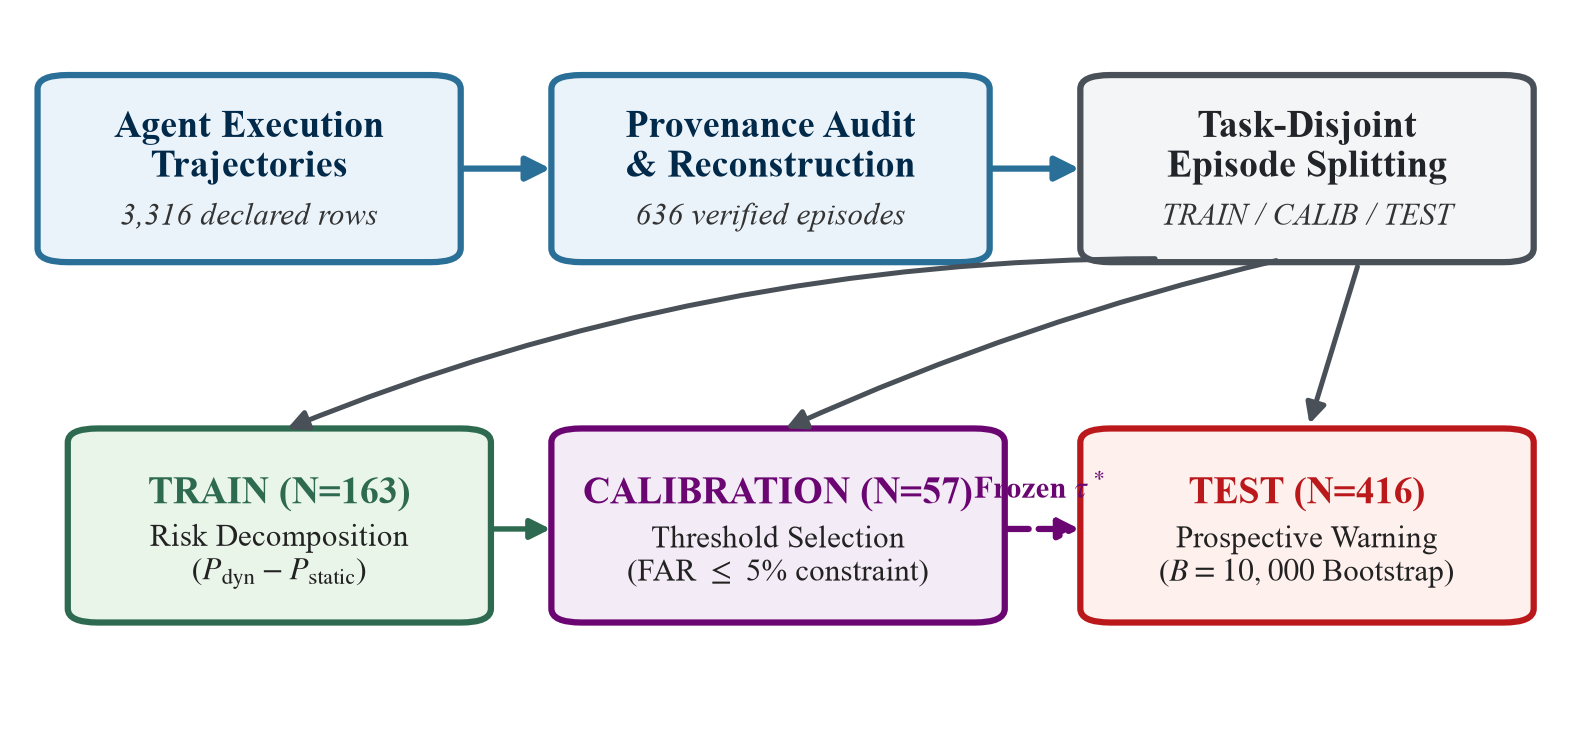
\includegraphics[keepaspectratio,alt={Fig. 1. AIRE-Trace standardized prospective evaluation pipeline. Trajectories are provenance-audited before episode-level splitting; trainable methods are fitted on TRAIN, operating thresholds are selected on CALIBRATION under the false-alarm constraint, and frozen thresholds are applied to the TEST population for prospective evaluation and operational analysis.}]{figures/ieee/fig1_aire_trace_architecture.png}}
\caption{Fig. 1. AIRE-Trace standardized prospective evaluation
pipeline. Trajectories are provenance-audited before episode-level
splitting; trainable methods are fitted on TRAIN, operating thresholds
are selected on CALIBRATION under the false-alarm constraint, and frozen
thresholds are applied to the TEST population for prospective evaluation
and operational analysis.}
\end{figure}

\subsubsection{D. Warning Formulation}\label{d.-warning-formulation}

Given a prefix at checkpoint t, a monitor produces a risk score
s(e1,\ldots,et) in {[}0,1{]}. An alert is raised when s \textgreater=
tau for a calibrated threshold tau.

Episode-level FAR (denominator = successful TEST episodes):

\begin{verbatim}
FAR = |{i : success(i), exists t: alert raised}| / |{i : success(i)}|
\end{verbatim}

\subsubsection{E. Evaluation Modes}\label{e.-evaluation-modes}

\textbf{Mode A -- Prospective-Warning Evaluation:} Conducted on
TerminalBench (failure-onset annotations present). Supports AUROC,
AUPRC, Brier, ECE, prospective Recall@FAR, lead time, and late-detection
analysis. Primary reported mode.

\textbf{Mode B -- Eventual-Outcome Diagnostic:} Conducted on tau2-Bench
(no onset annotations). Reports eventual-outcome ranking metrics only
(AUROC, AUPRC, Brier, ECE, Raw Recall). Does NOT support prospective
Recall@FAR. Mode B metrics must not be compared directly to Mode A
metrics.

\begin{center}\rule{0.5\linewidth}{0.5pt}\end{center}

\subsection{IV. Dataset, Provenance, and Study
Population}\label{iv.-dataset-provenance-and-study-population}

\subsubsection{A. Source Corpus}\label{a.-source-corpus}

Primary corpus: Tracebench (Contextbench/Tracebench) -- 3,316 declared
source rows, AI agent coding-task trajectory recordings.

Secondary corpus (Mode B only): tau2-Bench (sierra-research/tau-bench)
-- 1,980 episodes, 115 tasks, outcome-only (no onset annotations).

\textbf{Canonical Outcome Mapping (Protocol Rule 10):} - reward == 1.0 /
solved == True -\textgreater{} eventual\_success - reward == 0.0 /
solved == False -\textgreater{} eventual\_failure

\subsubsection{B. Provenance-Repair
Process}\label{b.-provenance-repair-process}

Source: post\_recovery\_audit.txt, lineage\_verification.txt.

State transitions applied to 3,316 declared rows: - 636 rows retained
(verified\_existing): valid mini.traj.json artifact present. - 2,655
rows excluded (structurally\_invalid): mini.traj.json absent after
artifact inspection. - 25 rows excluded (missing\_artifact\_path):
artifact path absent from source metadata.

\textbf{Recovery investigation:} 1,457 previously network-excluded
artifacts were successfully downloaded. Upon inspection, 100\% were
structurally invalid (mini.traj.json absent). Net addition to valid
population: 0.

\textbf{Final valid population: 636 episodes (19.18\% of 3,316 declared
rows).}

All downstream results are valid for this 636-episode population only.

The provenance and exclusion accounting leading to this subset is
detailed in Fig. 2.

\begin{figure}
\centering
\pandocbounded{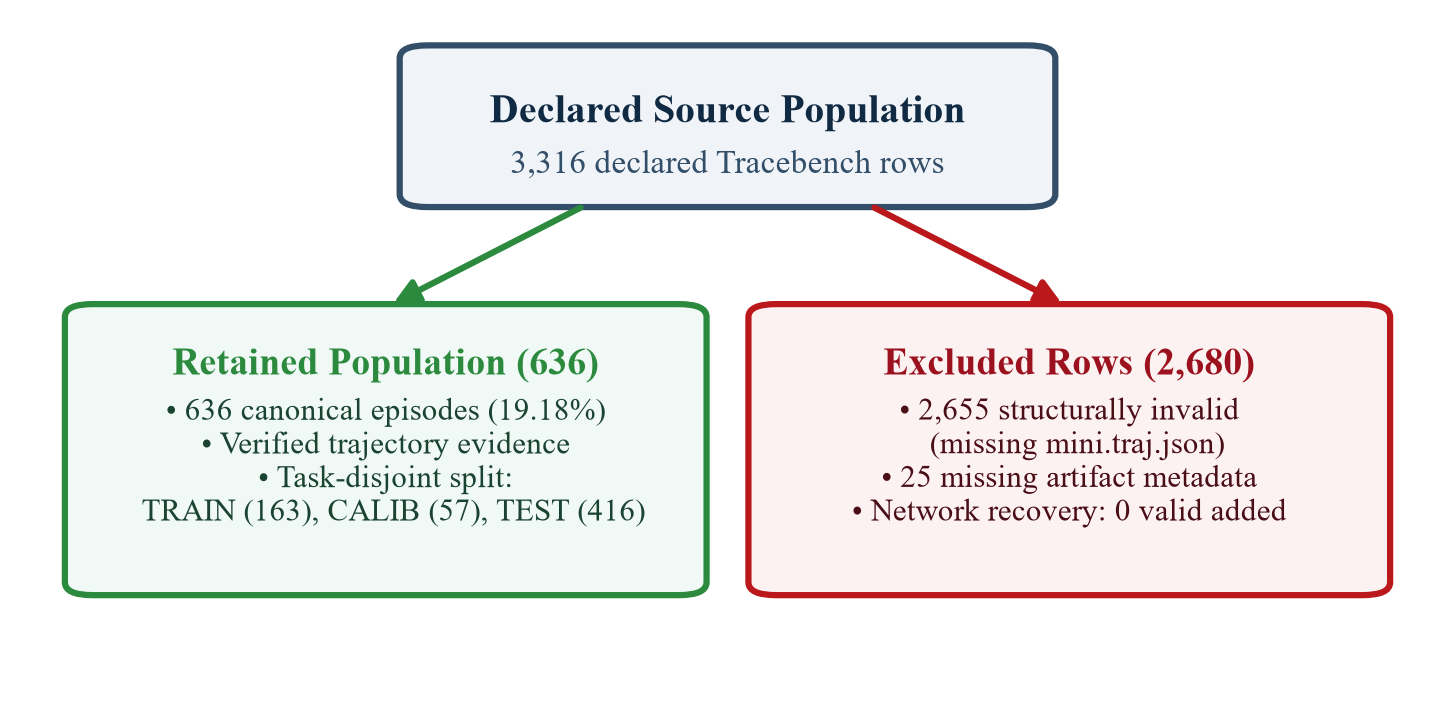
\includegraphics[keepaspectratio,alt={Fig. 2. Provenance and exclusion accounting for the AIRE-Trace empirical population. The downstream study is restricted to the canonical 636-episode population for which the required trajectory evidence was verified or deterministically reconstructed.}]{figures/ieee/fig2_provenance_recovery.png}}
\caption{Fig. 2. Provenance and exclusion accounting for the AIRE-Trace
empirical population. The downstream study is restricted to the
canonical 636-episode population for which the required trajectory
evidence was verified or deterministically reconstructed.}
\end{figure}

\subsubsection{C. Sanitization}\label{c.-sanitization}

Terminal event content replaced with redaction marker before any feature
extraction. Outcome keys stripped from trace feature inputs. (Protocol
Rule 6.)

\subsubsection{D. Train/Calibration/Test
Split}\label{d.-traincalibrationtest-split}

Episode-level split (complete episode assigned to exactly one split):

{\def\LTcaptype{none} % do not increment counter
\begin{longtable}[]{@{}lll@{}}
\toprule\noalign{}
Split & Episodes & Source \\
\midrule\noalign{}
\endhead
\bottomrule\noalign{}
\endlastfoot
TRAIN & 163 & gate7\_ablation.json A0 \\
CALIBRATION & 57 & gate7\_ablation.json A0 \\
TEST & 416 & primary\_k30\_results.json \\
Total & 636 & \\
\end{longtable}
}

\subsubsection{E. TEST Population
Accounting}\label{e.-test-population-accounting}

{\def\LTcaptype{none} % do not increment counter
\begin{longtable}[]{@{}
  >{\raggedright\arraybackslash}p{(\linewidth - 4\tabcolsep) * \real{0.4125}}
  >{\raggedright\arraybackslash}p{(\linewidth - 4\tabcolsep) * \real{0.0875}}
  >{\raggedright\arraybackslash}p{(\linewidth - 4\tabcolsep) * \real{0.5000}}@{}}
\toprule\noalign{}
\begin{minipage}[b]{\linewidth}\raggedright
Category
\end{minipage} & \begin{minipage}[b]{\linewidth}\raggedright
Count
\end{minipage} & \begin{minipage}[b]{\linewidth}\raggedright
Notes
\end{minipage} \\
\midrule\noalign{}
\endhead
\bottomrule\noalign{}
\endlastfoot
Total TEST episodes & 416 & Eligible for all ranking metrics \\
Failed TEST episodes & 317 & primary\_k30\_results.json \\
Successful TEST episodes & 99 & 416 - 317; FAR denominator \\
Valid annotated failure episodes & 257 & Recall@FAR and late-detection
denom \\
Unannotated failure episodes & 60 & Excluded from onset-dependent
metrics \\
Malformed onset episodes & 0 & \\
\end{longtable}
}

Source: primary\_k30\_results.json Exclusion\_Stats (consistent across
all 7 models).

\begin{center}\rule{0.5\linewidth}{0.5pt}\end{center}

\subsection{V. AIRE-Trace Evaluation
Protocol}\label{v.-aire-trace-evaluation-protocol}

\subsubsection{A. Feature Set (13 Category-A
Features)}\label{a.-feature-set-13-category-a-features}

{\def\LTcaptype{none} % do not increment counter
\begin{longtable}[]{@{}
  >{\raggedright\arraybackslash}p{(\linewidth - 2\tabcolsep) * \real{0.3867}}
  >{\raggedright\arraybackslash}p{(\linewidth - 2\tabcolsep) * \real{0.6133}}@{}}
\toprule\noalign{}
\begin{minipage}[b]{\linewidth}\raggedright
Feature
\end{minipage} & \begin{minipage}[b]{\linewidth}\raggedright
Description
\end{minipage} \\
\midrule\noalign{}
\endhead
\bottomrule\noalign{}
\endlastfoot
feat\_steps\_so\_far & Cumulative step count at checkpoint t \\
feat\_actor\_role\_agent & Count of agent-role events in prefix \\
feat\_actor\_role\_tool & Count of tool-role events in prefix \\
feat\_actor\_role\_user & Count of user-role events in prefix \\
feat\_actor\_role\_system & Count of system-role events in prefix \\
feat\_action\_type\_message & Count of message-type actions in prefix \\
feat\_action\_type\_tool\_call & Count of tool-call actions in prefix \\
feat\_action\_type\_tool\_result & Count of tool-result actions in
prefix \\
feat\_tool\_error\_count & Cumulative tool error count in prefix \\
feat\_retry\_count & Consecutive error sequence count in prefix \\
feat\_unique\_tools\_used & Number of distinct tools invoked in
prefix \\
feat\_tool\_call\_ratio & Ratio of tool calls to total actions \\
feat\_repeated\_action\_last2 & Indicator of repeated action in last 2
steps \\
\end{longtable}
}

Source: src/baselines/registry.py, gate7\_ablation.json (A0
retained\_features).

\subsubsection{B. Checkpoint Policy}\label{b.-checkpoint-policy}

t in \{1, \ldots, min(Ti, K)\}, K = 30. Outcome-independent,
episode-symmetric. Monitor accesses only e1,\ldots,et at inference time.

\subsubsection{C. Episode-Balanced
Weighting}\label{c.-episode-balanced-weighting}

w\_\{i,t\} = 1 / min(Ti, K). Ensures each episode contributes equally to
prefix-level metric computation regardless of trajectory length.

\subsubsection{D. Threshold Calibration}\label{d.-threshold-calibration}

Select tau* = argmax\_tau Recall(tau) subject to FAR\_calib(tau)
\textless= target\_FAR, on CALIBRATION split only. Ties: lower FAR
first, then higher threshold. tau* is frozen; TEST is not examined
before freeze. Target FAR for primary evaluation: 5\% (0.05).

Frozen thresholds (source: primary\_k30\_results.json,
calibrated\_thresholds.json):

{\def\LTcaptype{none} % do not increment counter
\begin{longtable}[]{@{}llll@{}}
\toprule\noalign{}
Model & Frozen Threshold & Calibration FAR & Calibration Recall \\
\midrule\noalign{}
\endhead
\bottomrule\noalign{}
\endlastfoot
H1 & 0.86 & 0.000 & 0.0263 \\
H2 & 0.89 & 0.000 & 0.0000 \\
H3 & 0.01 & 1.000 & 0.8158 \\
H4 & 0.93 & 0.000 & 0.0000 \\
M1 & 0.98 & 0.000 & 0.0000 \\
S1 & 0.97 & 0.000 & 0.0263 \\
S2 & 0.74 & 0.000 & 0.0000 \\
\end{longtable}
}

Note: H3 calibration FAR = 1.000 -- the 5\% FAR constraint was not
achievable on CALIBRATION. H3's Recall@FAR is undefined (NaN) in TEST
evaluation.

\subsubsection{E. Evaluation Metrics}\label{e.-evaluation-metrics}

Mode A -- prefix-level ranking (episode-balanced weights): AUROC, AUPRC,
Brier Score, ECE. Mode A -- episode-level operational: FAR (denominator:
N=99 successful TEST episodes), Recall@FAR (denominator: N=257 valid
annotated failure episodes). Mode B -- tau2-Bench diagnostic only: AUROC
(B), AUPRC (B), Brier (B), ECE (B), Raw Recall (B). Not comparable to
Mode A.

\begin{center}\rule{0.5\linewidth}{0.5pt}\end{center}

\subsection{VI. Warning Methods and
Implementation}\label{vi.-warning-methods-and-implementation}

\subsubsection{A. Heuristic Monitors (H1--H4) --
Training-Free}\label{a.-heuristic-monitors-h1h4-training-free}

\textbf{H1 -- Tool-Error Rate Monitor:} Risk score = min-max
normalization of feat\_tool\_error\_count across the evaluation batch.
Source: src/baselines/heuristics.py, HeuristicMonitor.

\textbf{H2 -- Retry-Count Monitor:} Risk score = min-max normalization
of feat\_retry\_count. Source: src/baselines/heuristics.py,
HeuristicMonitor.

\textbf{H3 -- Repeated-Action Monitor:} Risk score = min-max
normalization of feat\_repeated\_action\_last2. Effective threshold 0.01
caused calibration FAR = 1.000; operates outside the intended 5\% FAR
regime. Source: src/baselines/heuristics.py, HeuristicMonitor.

\textbf{H4 -- Combined Heuristic Monitor:} Risk score = sigmoid(average
z-score of feat\_tool\_error\_count, feat\_retry\_count,
feat\_repeated\_action\_last2). Z-score normalization parameters
computed on TRAIN only. Source: src/baselines/heuristics.py,
CombinedHeuristicMonitor.

\subsubsection{B. Classical Machine Learning Monitor
(M1)}\label{b.-classical-machine-learning-monitor-m1}

\textbf{M1 -- Logistic Regression:} scikit-learn LogisticRegression
(C=1.0, solver=lbfgs, max\_iter=1000, random\_state=42) over 13
Category-A features with StandardScaler normalization. Fitted on TRAIN
with episode-balanced sample weights. Source: src/baselines/logistic.py,
LogisticBaseline.

\subsubsection{C. Sequence Monitor S1 -- Random
Forest}\label{c.-sequence-monitor-s1-random-forest}

\textbf{S1 -- Random Forest Classifier:} scikit-learn
RandomForestClassifier (n\_estimators=100, max\_depth=6,
min\_samples\_split=5, random\_state=42) over 13 Category-A features. No
input normalization. Fitted on TRAIN with episode-balanced sample
weights. Source: src/baselines/random\_forest.py, RandomForestBaseline.

NOTE: S1 is classified in the Sequence (S) family by the project
registry (src/baselines/registry.py) but implemented as a Random Forest
tabular ensemble, not a sequential recurrent model. The model-ID
assignment follows the frozen registry and is preserved as-is from the
frozen experimental setup.

\subsubsection{D. Sequence Monitor S2 --
GRU}\label{d.-sequence-monitor-s2-gru}

\textbf{S2 -- GRU Sequence Model:} PyTorch GRU network (hidden\_dim=64,
num\_layers=1, lr=1e-3, epochs=10, batch\_size=128, device=cpu,
random\_seed=42). 13 Category-A features normalized via StandardScaler.
BCEWithLogitsLoss with episode-balanced weights. Fitted on TRAIN
episodes. Source: src/baselines/sequence.py, SequenceBaseline.

\subsubsection{E. Placeholder Model L}\label{e.-placeholder-model-l}

\textbf{L -- Semantic/LLM Monitor:} Registered as L\_PENDING in
src/baselines/registry.py. Not empirically evaluated. Hardware
constraint (RTX 2050, 4GB VRAM) precluded protocol-compliant evaluation
over the full dataset. No L results are reported; no conclusions about
L's prospective performance can be drawn.

\begin{center}\rule{0.5\linewidth}{0.5pt}\end{center}

\subsection{VII. Experimental Protocol and Statistical
Analysis}\label{vii.-experimental-protocol-and-statistical-analysis}

\subsubsection{A. Experimental Setup}\label{a.-experimental-setup}

All experiments use random seed 42. The MasterEvaluator class
(src/evaluation/evaluator.py) programmatically enforces: prefix-horizon
cutoff at K=30, post-onset exclusion from Recall@FAR denominator,
episode-balanced weighting, CALIBRATION-only threshold selection and
freezing, and runtime leakage guards before any model fitting or
scoring.

\subsubsection{B. Bootstrap Confidence
Intervals}\label{b.-bootstrap-confidence-intervals}

Procedure: Paired episode-cluster bootstrap, B = 1,000 iterations.
Episodes resampled with replacement at the episode level (NOT prefix
level). Frozen thresholds held constant across resamples. 95\% CI:
2.5th--97.5th percentile of bootstrap distribution.

Why prefix-level resampling is incorrect: prefixes within the same
episode share the outcome label and co-vary in feature patterns,
violating the independence assumption and producing pseudo-replication
with artificially narrow CIs.

\subsubsection{C. Statistical Hypothesis
Testing}\label{c.-statistical-hypothesis-testing}

Family of comparisons: S1 vs.~\{M1, S2, H1, H2, H3, H4\} for AUROC and
AUPRC (12 total comparisons). H0: Delta(metric) = 0 between S1 and
comparator. Test statistic: observed metric difference Delta\_obs.
Null-centering: bootstrap differences are centered; p\_raw = proportion
\textbar Delta\_boot\textbar{} \textgreater=
\textbar Delta\_obs\textbar. Correction: Holm--Bonferroni step-down
across 6 comparisons per metric (AUROC and AUPRC separately), alpha =
0.05.

No p-values are fabricated. Significance claims are strictly limited to
what the bootstrap test results support.

\subsubsection{D. Pairwise Direction Consistency
(PDC)}\label{d.-pairwise-direction-consistency-pdc}

For each model pair (A,B): metric-comparison direction across AUROC,
AUPRC, Recall@FAR, ECE. PDC per pair = proportion of non-tied
comparisons with the majority direction. Coverage per pair = fraction of
metrics that are non-tied (informative). Overall PDC = mean PDC across
all informative pairs. PDC must always be reported with its coverage
figure.

\subsubsection{E. Feature Ablation Design
(Frozen)}\label{e.-feature-ablation-design-frozen}

Ablation matrix frozen per RESEARCH\_LOG.md (2026-08-10): - A0: All 13
features (full baseline) - A1: Remove feat\_steps\_so\_far - A2: Remove
4 actor-role features - A3: Remove 3 action-type features - A4: Remove
feat\_tool\_error\_count + feat\_retry\_count - A5: Remove
feat\_unique\_tools\_used + feat\_tool\_call\_ratio - A6: Remove
feat\_repeated\_action\_last2

Each ablation uses identical MasterEvaluator with re-calibration on
CALIBRATION and metrics on TEST. No TEST outcomes are used for ablation
design or selection.

\subsubsection{F. FAR Sensitivity
Analysis}\label{f.-far-sensitivity-analysis}

S1 evaluated at target FAR = \{1\%, 5\%, 10\%\}. AUROC and AUPRC are
threshold-independent and unchanged across FAR targets. Only frozen
threshold, TEST FAR, and Recall@FAR change.

\begin{center}\rule{0.5\linewidth}{0.5pt}\end{center}

\subsection{VIII. Results}\label{viii.-results}

\subsubsection{A. TABLE I -- Study Population
Accounting}\label{a.-table-i-study-population-accounting}

{\def\LTcaptype{none} % do not increment counter
\begin{longtable}[]{@{}
  >{\raggedright\arraybackslash}p{(\linewidth - 4\tabcolsep) * \real{0.4783}}
  >{\raggedright\arraybackslash}p{(\linewidth - 4\tabcolsep) * \real{0.1304}}
  >{\raggedright\arraybackslash}p{(\linewidth - 4\tabcolsep) * \real{0.3913}}@{}}
\toprule\noalign{}
\begin{minipage}[b]{\linewidth}\raggedright
Quantity
\end{minipage} & \begin{minipage}[b]{\linewidth}\raggedright
Count
\end{minipage} & \begin{minipage}[b]{\linewidth}\raggedright
Source
\end{minipage} \\
\midrule\noalign{}
\endhead
\bottomrule\noalign{}
\endlastfoot
Declared Tracebench rows & 3,316 & post\_recovery\_audit.txt \\
Valid reconstructed episodes & 636 & post\_recovery\_audit.txt \\
Structurally invalid & 2,655 & post\_recovery\_audit.txt \\
Missing artifact path & 25 & post\_recovery\_audit.txt \\
Coverage (636/3316) & 19.18\% & Computed \\
TRAIN episodes & 163 & gate7\_ablation.json (A0) \\
CALIBRATION episodes & 57 & gate7\_ablation.json (A0) \\
TEST episodes & 416 & primary\_k30\_results.json \\
TEST: failed episodes & 317 & primary\_k30\_results.json \\
TEST: successful episodes & 99 & 416 - 317 \\
TEST: valid annotated failures & 257 & primary\_k30\_results.json \\
TEST: unannotated failures & 60 & primary\_k30\_results.json \\
\end{longtable}
}

\subsubsection{B. TABLE II -- Warning Method
Definitions}\label{b.-table-ii-warning-method-definitions}

{\def\LTcaptype{none} % do not increment counter
\begin{longtable}[]{@{}
  >{\raggedright\arraybackslash}p{(\linewidth - 6\tabcolsep) * \real{0.0778}}
  >{\raggedright\arraybackslash}p{(\linewidth - 6\tabcolsep) * \real{0.1333}}
  >{\raggedright\arraybackslash}p{(\linewidth - 6\tabcolsep) * \real{0.3111}}
  >{\raggedright\arraybackslash}p{(\linewidth - 6\tabcolsep) * \real{0.4778}}@{}}
\toprule\noalign{}
\begin{minipage}[b]{\linewidth}\raggedright
Model
\end{minipage} & \begin{minipage}[b]{\linewidth}\raggedright
Family
\end{minipage} & \begin{minipage}[b]{\linewidth}\raggedright
Method
\end{minipage} & \begin{minipage}[b]{\linewidth}\raggedright
Key Parameters
\end{minipage} \\
\midrule\noalign{}
\endhead
\bottomrule\noalign{}
\endlastfoot
H1 & Heuristic & Tool-error rate monitor & Min-max
feat\_tool\_error\_count \\
H2 & Heuristic & Retry-count monitor & Min-max feat\_retry\_count \\
H3 & Heuristic & Repeated-action monitor & Min-max
feat\_repeated\_action\_last2 \\
H4 & Heuristic & Combined heuristic & sigmoid(z-score avg, 3
features) \\
M1 & Classical & Logistic Regression & C=1.0, lbfgs, StandardScaler,
seed=42 \\
S1 & Sequence* & Random Forest & n\_estimators=100, max\_depth=6,
seed=42 \\
S2 & Sequence & GRU & hidden\_dim=64, 1 layer, epochs=10, seed=42 \\
L & Semantic & LLM Monitor & NOT EVALUATED (hardware constraint) \\
\end{longtable}
}

*S1 classified Sequence by registry; implemented as Random Forest
tabular ensemble.

\subsubsection{C. TABLE III -- Primary Mode A TEST Performance (K=30,
target FAR
5\%)}\label{c.-table-iii-primary-mode-a-test-performance-k30-target-far-5}

All values LEVEL 1 evidence. Source: baseline\_comparison\_table.csv,
primary\_k30\_results.json.

{\def\LTcaptype{none} % do not increment counter
\begin{longtable}[]{@{}
  >{\raggedright\arraybackslash}p{(\linewidth - 20\tabcolsep) * \real{0.0579}}
  >{\raggedright\arraybackslash}p{(\linewidth - 20\tabcolsep) * \real{0.0661}}
  >{\raggedright\arraybackslash}p{(\linewidth - 20\tabcolsep) * \real{0.1488}}
  >{\raggedright\arraybackslash}p{(\linewidth - 20\tabcolsep) * \real{0.0661}}
  >{\raggedright\arraybackslash}p{(\linewidth - 20\tabcolsep) * \real{0.1488}}
  >{\raggedright\arraybackslash}p{(\linewidth - 20\tabcolsep) * \real{0.0992}}
  >{\raggedright\arraybackslash}p{(\linewidth - 20\tabcolsep) * \real{0.1488}}
  >{\raggedright\arraybackslash}p{(\linewidth - 20\tabcolsep) * \real{0.0826}}
  >{\raggedright\arraybackslash}p{(\linewidth - 20\tabcolsep) * \real{0.0661}}
  >{\raggedright\arraybackslash}p{(\linewidth - 20\tabcolsep) * \real{0.0661}}
  >{\raggedright\arraybackslash}p{(\linewidth - 20\tabcolsep) * \real{0.0496}}@{}}
\toprule\noalign{}
\begin{minipage}[b]{\linewidth}\raggedright
Model
\end{minipage} & \begin{minipage}[b]{\linewidth}\raggedright
AUROC
\end{minipage} & \begin{minipage}[b]{\linewidth}\raggedright
95\% CI
\end{minipage} & \begin{minipage}[b]{\linewidth}\raggedright
AUPRC
\end{minipage} & \begin{minipage}[b]{\linewidth}\raggedright
95\% CI
\end{minipage} & \begin{minipage}[b]{\linewidth}\raggedright
Recall@FAR
\end{minipage} & \begin{minipage}[b]{\linewidth}\raggedright
95\% CI
\end{minipage} & \begin{minipage}[b]{\linewidth}\raggedright
TEST FAR
\end{minipage} & \begin{minipage}[b]{\linewidth}\raggedright
Brier
\end{minipage} & \begin{minipage}[b]{\linewidth}\raggedright
ECE
\end{minipage} & \begin{minipage}[b]{\linewidth}\raggedright
tau
\end{minipage} \\
\midrule\noalign{}
\endhead
\bottomrule\noalign{}
\endlastfoot
H1 & 0.6205 & {[}0.5799, 0.6513{]} & 0.8371 & {[}0.7894, 0.8674{]} &
0.0000 & {[}0.0000, 0.0000{]} & 0.0000 & 0.6186 & 0.6622 & 0.86 \\
H2 & 0.5752 & {[}0.5402, 0.6116{]} & 0.8329 & {[}0.7799, 0.8702{]} &
0.0000 & {[}0.0000, 0.0000{]} & 0.0000 & 0.7034 & 0.7223 & 0.89 \\
H3 & 0.5074 & {[}0.5024, 0.5122{]} & 0.8702 & {[}0.8476, 0.8927{]} &
UNDEF & (see note) & 1.0000 & 0.2885 & 0.2885 & 0.01 \\
H4 & 0.6135 & {[}0.5729, 0.6445{]} & 0.8346 & {[}0.7866, 0.8647{]} &
0.0000 & {[}0.0000, 0.0000{]} & 0.0202 & 0.2644 & 0.2794 & 0.93 \\
M1 & 0.6215 & {[}0.5630, 0.6629{]} & 0.8331 & {[}0.7796, 0.8659{]} &
0.0078 & {[}0.0000, 0.0195{]} & 0.0303 & 0.1767 & 0.0140 & 0.98 \\
S1 & 0.6371 & {[}0.5885, 0.6745{]} & 0.8452 & {[}0.8020, 0.8761{]} &
0.0000 & {[}0.0000, 0.0000{]} & 0.0404 & 0.1746 & 0.0124 & 0.97 \\
S2 & 0.5496 & {[}0.5212, 0.5734{]} & 0.8129 & {[}0.7638, 0.8436{]} &
0.0000 & {[}0.0000, 0.0000{]} & 0.0000 & 0.2042 & 0.1530 & 0.74 \\
\end{longtable}
}

Note: H3 Recall@FAR is undefined (NaN) because calibration FAR reached
1.000 -- the 5\% constraint was not achievable on CALIBRATION. This
metric is uninformative for H3.

\textbf{Mode B results (tau2-Bench, NOT comparable to Mode A):}

Source: primary\_k30\_results.json mode\_b\_tau2\_bench. LEVEL 1
evidence.

{\def\LTcaptype{none} % do not increment counter
\begin{longtable}[]{@{}
  >{\raggedright\arraybackslash}p{(\linewidth - 12\tabcolsep) * \real{0.1029}}
  >{\raggedright\arraybackslash}p{(\linewidth - 12\tabcolsep) * \real{0.1471}}
  >{\raggedright\arraybackslash}p{(\linewidth - 12\tabcolsep) * \real{0.1471}}
  >{\raggedright\arraybackslash}p{(\linewidth - 12\tabcolsep) * \real{0.1471}}
  >{\raggedright\arraybackslash}p{(\linewidth - 12\tabcolsep) * \real{0.1176}}
  >{\raggedright\arraybackslash}p{(\linewidth - 12\tabcolsep) * \real{0.1176}}
  >{\raggedright\arraybackslash}p{(\linewidth - 12\tabcolsep) * \real{0.2206}}@{}}
\toprule\noalign{}
\begin{minipage}[b]{\linewidth}\raggedright
Model
\end{minipage} & \begin{minipage}[b]{\linewidth}\raggedright
AUROC(B)
\end{minipage} & \begin{minipage}[b]{\linewidth}\raggedright
AUPRC(B)
\end{minipage} & \begin{minipage}[b]{\linewidth}\raggedright
Brier(B)
\end{minipage} & \begin{minipage}[b]{\linewidth}\raggedright
ECE(B)
\end{minipage} & \begin{minipage}[b]{\linewidth}\raggedright
FAR(B)
\end{minipage} & \begin{minipage}[b]{\linewidth}\raggedright
Raw Recall(B)
\end{minipage} \\
\midrule\noalign{}
\endhead
\bottomrule\noalign{}
\endlastfoot
H1 & 0.5000 & 0.7013 & 0.4025 & 0.4025 & 0.0000 & 0.0000 \\
H2 & 0.5000 & 0.7013 & 0.4025 & 0.4025 & 0.0000 & 0.0000 \\
H3 & 0.5027 & 0.5417 & 0.4892 & 0.4892 & 1.0000 & 1.0000 \\
H4 & 0.5027 & 0.5417 & 0.2640 & 0.1223 & 0.0000 & 0.0000 \\
M1 & 0.5233 & 0.4436 & 0.5843 & 0.5846 & 1.0000 & 1.0000 \\
S1 & 0.5029 & 0.4026 & 0.3892 & 0.3849 & 0.0000 & 0.0000 \\
S2 & 0.5300 & 0.4318 & 0.2474 & 0.0867 & 0.0000 & 0.0000 \\
\end{longtable}
}

The performance results are visually summarized in Fig. 4.

\begin{figure}
\centering
\pandocbounded{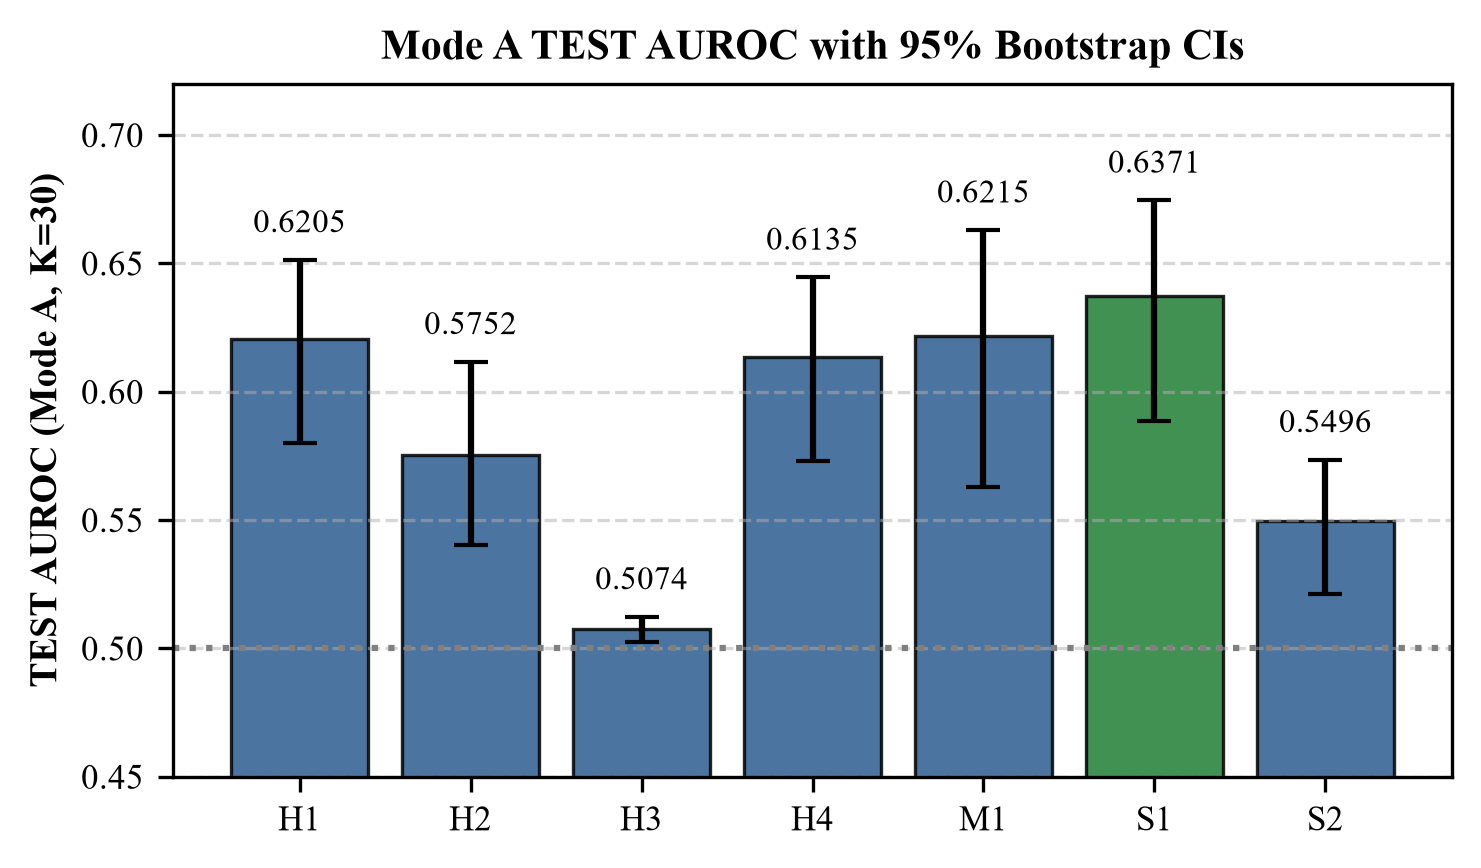
\includegraphics[keepaspectratio,alt={Fig. 4. Mode A TEST AUROC for the evaluated warning methods under the K=30 protocol. Error bars denote the corresponding 95\% episode-cluster bootstrap confidence intervals.}]{figures/ieee/fig4_mode_a_auroc.png}}
\caption{Fig. 4. Mode A TEST AUROC for the evaluated warning methods
under the K=30 protocol. Error bars denote the corresponding 95\%
episode-cluster bootstrap confidence intervals.}
\end{figure}

\subsubsection{D. TABLE V -- Statistical Tests (S1 vs.~comparators,
B=1000,
Holm-Bonferroni)}\label{d.-table-v-statistical-tests-s1-vs.-comparators-b1000-holm-bonferroni}

Source: reports/gate7\_statistical\_tests.json. LEVEL 1 evidence.

{\def\LTcaptype{none} % do not increment counter
\begin{longtable}[]{@{}
  >{\raggedright\arraybackslash}p{(\linewidth - 10\tabcolsep) * \real{0.1765}}
  >{\raggedright\arraybackslash}p{(\linewidth - 10\tabcolsep) * \real{0.1176}}
  >{\raggedright\arraybackslash}p{(\linewidth - 10\tabcolsep) * \real{0.1618}}
  >{\raggedright\arraybackslash}p{(\linewidth - 10\tabcolsep) * \real{0.1176}}
  >{\raggedright\arraybackslash}p{(\linewidth - 10\tabcolsep) * \real{0.1176}}
  >{\raggedright\arraybackslash}p{(\linewidth - 10\tabcolsep) * \real{0.3088}}@{}}
\toprule\noalign{}
\begin{minipage}[b]{\linewidth}\raggedright
Comparison
\end{minipage} & \begin{minipage}[b]{\linewidth}\raggedright
Metric
\end{minipage} & \begin{minipage}[b]{\linewidth}\raggedright
Delta\_obs
\end{minipage} & \begin{minipage}[b]{\linewidth}\raggedright
p\_raw
\end{minipage} & \begin{minipage}[b]{\linewidth}\raggedright
p\_adj
\end{minipage} & \begin{minipage}[b]{\linewidth}\raggedright
Reject H0 (a=0.05)
\end{minipage} \\
\midrule\noalign{}
\endhead
\bottomrule\noalign{}
\endlastfoot
S1 vs M1 & AUROC & +0.0156 & 0.1588 & 0.3177 & No \\
S1 vs S2 & AUROC & +0.0875 & 0.0010 & 0.0060 & YES \\
S1 vs H1 & AUROC & +0.0165 & 0.1948 & 0.3177 & No \\
S1 vs H2 & AUROC & +0.0619 & 0.0010 & 0.0060 & YES \\
S1 vs H3 & AUROC & +0.1297 & 0.0010 & 0.0060 & YES \\
S1 vs H4 & AUROC & +0.0236 & 0.0559 & 0.1678 & No \\
S1 vs M1 & AUPRC & +0.0121 & 0.0849 & 0.4246 & No \\
S1 vs S2 & AUPRC & +0.0323 & 0.0020 & 0.0120 & YES \\
S1 vs H1 & AUPRC & +0.0082 & 0.2517 & 0.4246 & No \\
S1 vs H2 & AUPRC & +0.0124 & 0.1538 & 0.4246 & No \\
S1 vs H3 & AUPRC & -0.0250 & 0.0919 & 0.4246 & No \\
S1 vs H4 & AUPRC & +0.0106 & 0.1189 & 0.4246 & No \\
\end{longtable}
}

Key findings: - S1 statistically significant AUROC advantages: S2, H2,
H3 (p\_adj = 0.006 each). - S1 NOT significant vs.: M1, H1, H4 (AUROC);
M1, H1, H2, H3, H4 (AUPRC). - S1 statistically significant AUPRC
advantage: S2 only (p\_adj = 0.012). - H3 showed directionally favorable
AUPRC point estimate vs.~S1 (Delta\_obs = -0.0250, not significant). -
S1's advantages are selective, not universal.

\subsubsection{E. Pairwise Direction Consistency
(PDC)}\label{e.-pairwise-direction-consistency-pdc}

Source: results/baseline\_runs/pdc\_summary.json. LEVEL 1 evidence.

Overall PDC: 0.8294 Coverage: 0.881 Total pairs: 21; Informative pairs:
21 of 21.

PDC of 0.8294 indicates that across the evaluated metric set, the
majority of pairwise ranking directions are consistent, while
approximately 17\% of informative comparisons contain at least one
metric disagreement.

\subsubsection{F. Operating-Point Sensitivity
(S1)}\label{f.-operating-point-sensitivity-s1}

Source: reports/gate7\_far\_sensitivity.json. LEVEL 1 evidence.

{\def\LTcaptype{none} % do not increment counter
\begin{longtable}[]{@{}
  >{\raggedright\arraybackslash}p{(\linewidth - 8\tabcolsep) * \real{0.1791}}
  >{\raggedright\arraybackslash}p{(\linewidth - 8\tabcolsep) * \real{0.2537}}
  >{\raggedright\arraybackslash}p{(\linewidth - 8\tabcolsep) * \real{0.1642}}
  >{\raggedright\arraybackslash}p{(\linewidth - 8\tabcolsep) * \real{0.1493}}
  >{\raggedright\arraybackslash}p{(\linewidth - 8\tabcolsep) * \real{0.2537}}@{}}
\toprule\noalign{}
\begin{minipage}[b]{\linewidth}\raggedright
Target FAR
\end{minipage} & \begin{minipage}[b]{\linewidth}\raggedright
Frozen Threshold
\end{minipage} & \begin{minipage}[b]{\linewidth}\raggedright
Calib FAR
\end{minipage} & \begin{minipage}[b]{\linewidth}\raggedright
TEST FAR
\end{minipage} & \begin{minipage}[b]{\linewidth}\raggedright
TEST Recall@FAR
\end{minipage} \\
\midrule\noalign{}
\endhead
\bottomrule\noalign{}
\endlastfoot
1\% & 0.97 & 0.00 & 0.0404 & 0.0000 \\
5\% & 0.97 & 0.00 & 0.0404 & 0.0000 \\
10\% & 0.93 & 0.10 & 0.1212 & 0.0973 \\
\end{longtable}
}

At 1\% and 5\% FAR targets, the calibration procedure selected the same
threshold (0.97). AUROC (0.6371) and AUPRC (0.8452) are
threshold-independent and unchanged across all three FAR levels.

\subsubsection{G. TABLE VI -- Feature Ablation Results (S1, Mode A,
K=30)}\label{g.-table-vi-feature-ablation-results-s1-mode-a-k30}

Source: reports/gate7\_ablation.json. LEVEL 1 evidence.

{\def\LTcaptype{none} % do not increment counter
\begin{longtable}[]{@{}
  >{\raggedright\arraybackslash}p{(\linewidth - 8\tabcolsep) * \real{0.0465}}
  >{\raggedright\arraybackslash}p{(\linewidth - 8\tabcolsep) * \real{0.5465}}
  >{\raggedright\arraybackslash}p{(\linewidth - 8\tabcolsep) * \real{0.1279}}
  >{\raggedright\arraybackslash}p{(\linewidth - 8\tabcolsep) * \real{0.1279}}
  >{\raggedright\arraybackslash}p{(\linewidth - 8\tabcolsep) * \real{0.1512}}@{}}
\toprule\noalign{}
\begin{minipage}[b]{\linewidth}\raggedright
ID
\end{minipage} & \begin{minipage}[b]{\linewidth}\raggedright
Removed Features
\end{minipage} & \begin{minipage}[b]{\linewidth}\raggedright
TEST AUROC
\end{minipage} & \begin{minipage}[b]{\linewidth}\raggedright
TEST AUPRC
\end{minipage} & \begin{minipage}[b]{\linewidth}\raggedright
Delta\_AUROC
\end{minipage} \\
\midrule\noalign{}
\endhead
\bottomrule\noalign{}
\endlastfoot
A0 & None (full baseline) & 0.6371 & 0.8452 & 0.0000 \\
A1 & feat\_steps\_so\_far & 0.6357 & 0.8450 & -0.0014 \\
A2 & 4 actor-role features & 0.6335 & 0.8422 & -0.0036 \\
A3 & 3 action-type features & 0.6383 & 0.8477 & +0.0012 \\
A4 & feat\_tool\_error\_count + feat\_retry\_count & 0.5302 & 0.7820 &
-0.1069 \\
A5 & feat\_unique\_tools\_used + feat\_tool\_call\_ratio & 0.6360 &
0.8479 & -0.0011 \\
A6 & feat\_repeated\_action\_last2 & 0.6341 & 0.8462 & -0.0030 \\
\end{longtable}
}

As shown in Fig. 5, a4 produced the largest observed degradation
(delta\_auroc = -0.1069). This establishes an association between
error/retry signals and discrimination performance; it does not
establish causality.

\begin{figure}
\centering
\pandocbounded{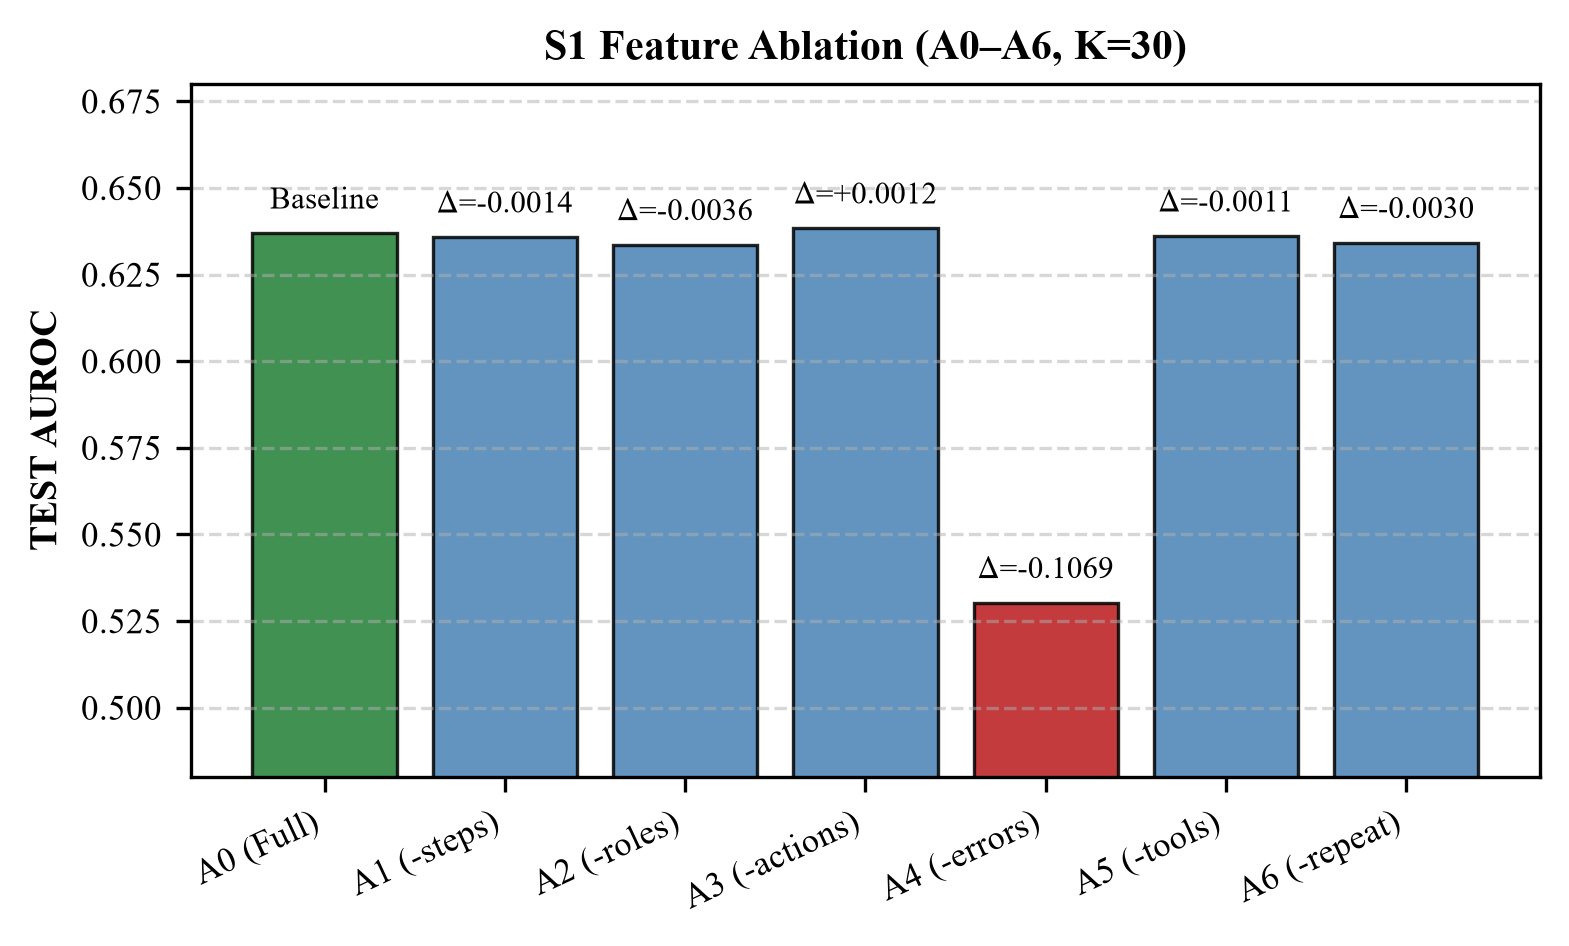
\includegraphics[keepaspectratio,alt={Fig. 5. A4 component ablation under the defined evaluation protocol. The observed AUROC change is reported as an empirical association under the ablation design and does not establish causal attribution.}]{figures/ieee/fig5_a4_ablation.png}}
\caption{Fig. 5. A4 component ablation under the defined evaluation
protocol. The observed AUROC change is reported as an empirical
association under the ablation design and does not establish causal
attribution.}
\end{figure}

\begin{center}\rule{0.5\linewidth}{0.5pt}\end{center}

\subsection{IX. Operational Analysis (Gate
6)}\label{ix.-operational-analysis-gate-6}

\subsubsection{A. TABLE IV -- Gate 6 Operational
Summary}\label{a.-table-iv-gate-6-operational-summary}

Sources: gate6\_false\_alarms.json, gate6\_late\_detections.json,
gate6\_alert\_burden.json. LEVEL 1 evidence. FAR denominator: 99
successful TEST episodes. Late-only denominator: 257 valid annotated
failure episodes. Total alerts denominator: 416 TEST episodes.

{\def\LTcaptype{none} % do not increment counter
\begin{longtable}[]{@{}
  >{\raggedright\arraybackslash}p{(\linewidth - 12\tabcolsep) * \real{0.0737}}
  >{\raggedright\arraybackslash}p{(\linewidth - 12\tabcolsep) * \real{0.1368}}
  >{\raggedright\arraybackslash}p{(\linewidth - 12\tabcolsep) * \real{0.1263}}
  >{\raggedright\arraybackslash}p{(\linewidth - 12\tabcolsep) * \real{0.2105}}
  >{\raggedright\arraybackslash}p{(\linewidth - 12\tabcolsep) * \real{0.1579}}
  >{\raggedright\arraybackslash}p{(\linewidth - 12\tabcolsep) * \real{0.1474}}
  >{\raggedright\arraybackslash}p{(\linewidth - 12\tabcolsep) * \real{0.1474}}@{}}
\toprule\noalign{}
\begin{minipage}[b]{\linewidth}\raggedright
Model
\end{minipage} & \begin{minipage}[b]{\linewidth}\raggedright
FA Episodes
\end{minipage} & \begin{minipage}[b]{\linewidth}\raggedright
FAR (N=99)
\end{minipage} & \begin{minipage}[b]{\linewidth}\raggedright
Late-Only Episodes
\end{minipage} & \begin{minipage}[b]{\linewidth}\raggedright
\% Valid Fails
\end{minipage} & \begin{minipage}[b]{\linewidth}\raggedright
Total Alerts
\end{minipage} & \begin{minipage}[b]{\linewidth}\raggedright
Mean/Episode
\end{minipage} \\
\midrule\noalign{}
\endhead
\bottomrule\noalign{}
\endlastfoot
H1 & 0 & 0.0000 & 3 & 1.17\% & 19 & 0.046 \\
H2 & 0 & 0.0000 & 2 & 0.78\% & 16 & 0.039 \\
H3 & 99 & 1.0000 & 51 & 19.84\% & 8,012 & 19.26 \\
H4 & 2 & 0.0202 & 8 & 3.11\% & 119 & 0.286 \\
M1 & 3 & 0.0303 & 10 & 3.89\% & 161 & 0.387 \\
S1 & 4 & 0.0404 & 16 & 6.23\% & 25 & 0.060 \\
S2 & 0 & 0.0000 & 10 & 3.89\% & 107 & 0.257 \\
\end{longtable}
}

These operational findings, highlighting false alarms, late-alert-only
episodes, and alert burden, are visualized in Fig. 6.

\begin{figure}
\centering
\pandocbounded{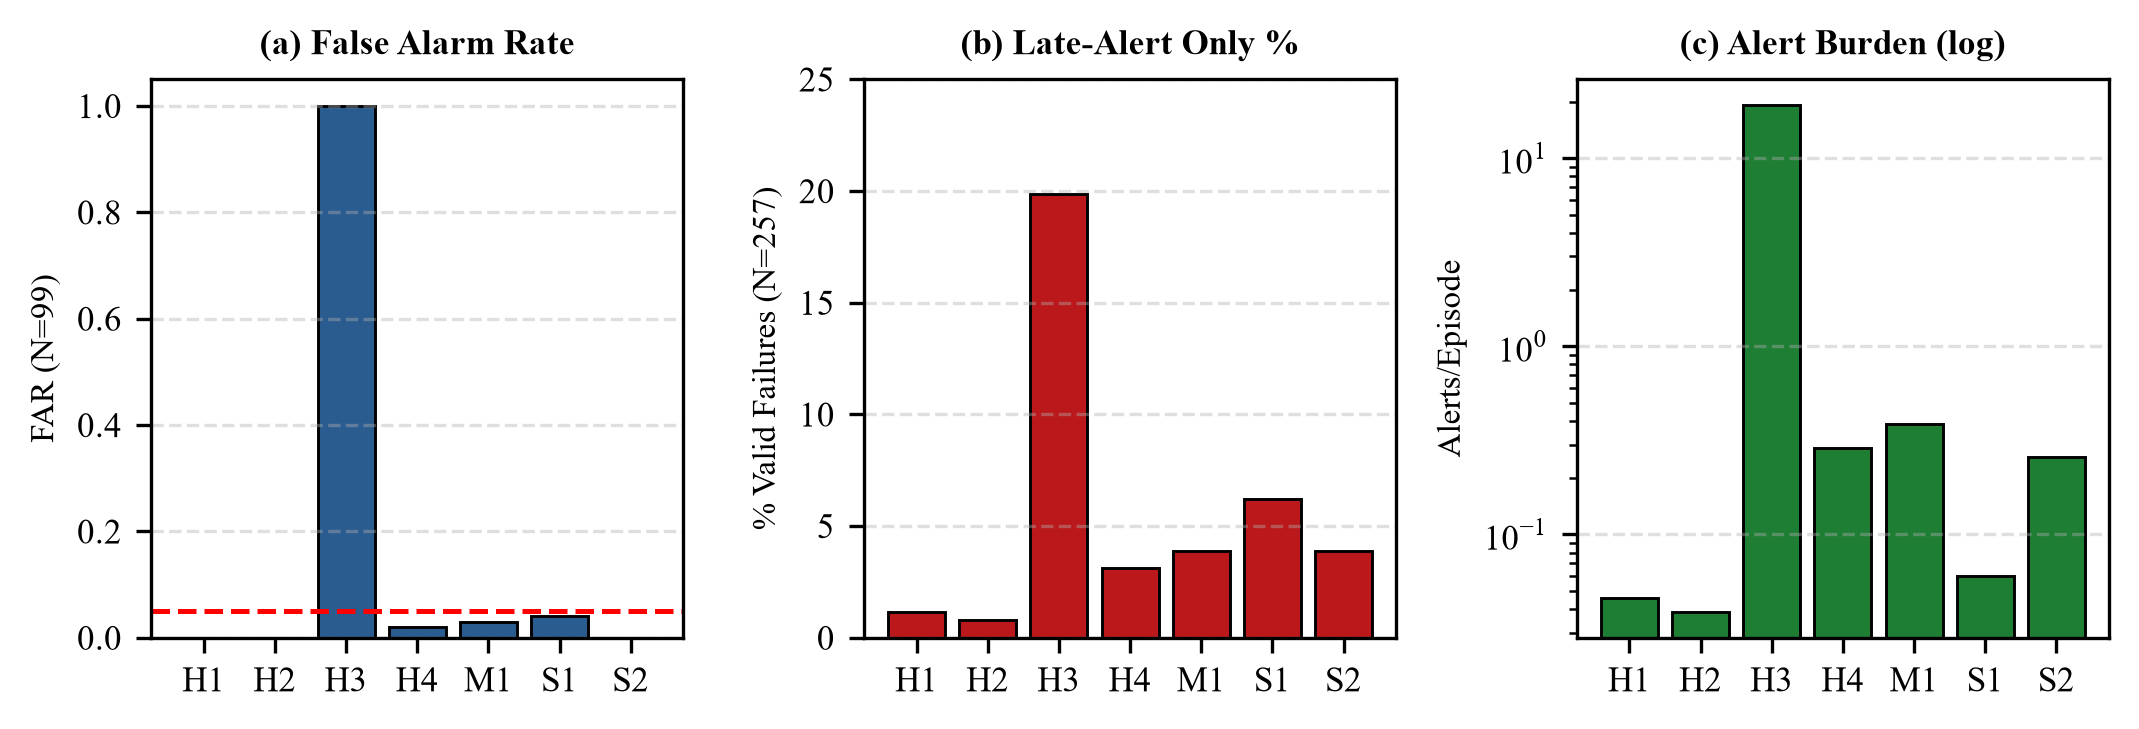
\includegraphics[keepaspectratio,alt={Fig. 6. Gate 6 operational analysis showing false alarms, late-alert-only episodes, and alert burden under the frozen TEST evaluation.}]{figures/ieee/fig6_gate6_operational.png}}
\caption{Fig. 6. Gate 6 operational analysis showing false alarms,
late-alert-only episodes, and alert burden under the frozen TEST
evaluation.}
\end{figure}

\subsubsection{B. Late Detections}\label{b.-late-detections}

An alert at t \textgreater{} t\_onset is a late detection and does not
constitute actionable prospective early warning.

Key findings (gate6\_late\_detections.json): - H3: 3,339 late alerts;
51/257 valid failure episodes (19.84\%) received ONLY late alerts. Mean
lateness: 9.15 steps; median: 8.0 steps. - S1: 19 late alerts; 16/257
(6.23\%) received only late alerts. Mean lateness: 17.84 steps; median:
17.0 steps. - H1: 3 late-alert-only episodes (1.17\%), mean lateness
25.89 steps. - H2: 2 late-alert-only episodes (0.78\%), mean lateness
25.50 steps. - H4: 8 (3.11\%); M1: 10 (3.89\%); S2: 10 (3.89\%).

\subsubsection{C. False Alarms}\label{c.-false-alarms}

Denominator: 99 successful TEST episodes.

Key findings (gate6\_false\_alarms.json): - H1, H2, S2: 0 false alarm
episodes (FAR = 0.000). - H4: 2 episodes (FAR = 0.0202). - M1: 3
episodes (FAR = 0.0303). - S1: 4 episodes (FAR = 4/99 = 0.0404). Episode
IDs: crack-7z-hash-6657a30e, install-klee-minimal-4b8b99db,
install-klee-minimal-776b2140, build-pov-ray-dddf443d. - H3: 99/99
episodes (FAR = 1.000). All successful episodes received at least one
alert.

S1 operational FAR (4.04\%) is within the 5\% target.

\subsubsection{D. Alert Burden}\label{d.-alert-burden}

Total alerts across all 416 TEST episodes (gate6\_alert\_burden.json):

{\def\LTcaptype{none} % do not increment counter
\begin{longtable}[]{@{}lllll@{}}
\toprule\noalign{}
Model & Total & Mean/Ep & Max/Ep & Zero-alert episodes \\
\midrule\noalign{}
\endhead
\bottomrule\noalign{}
\endlastfoot
H1 & 19 & 0.046 & 8 & 413/416 \\
H2 & 16 & 0.039 & 8 & 414/416 \\
H3 & 8,012 & 19.26 & 28 & 0/416 \\
H4 & 119 & 0.286 & 18 & 405/416 \\
M1 & 161 & 0.387 & 18 & 400/416 \\
S1 & 25 & 0.060 & 2 & 394/416 \\
S2 & 107 & 0.257 & 21 & 405/416 \\
\end{longtable}
}

S1 produced the lowest alert burden among models generating any
prospective detections (25 total; max 2 per episode).

\begin{center}\rule{0.5\linewidth}{0.5pt}\end{center}

\subsection{X. Discussion}\label{x.-discussion}

\subsubsection{A. The Operational Recall
Collapse}\label{a.-the-operational-recall-collapse}

S1's prospective Recall@FAR = 0.0000 at FAR \textless= 5\% indicates
that while the Random Forest achieves meaningful probabilistic
discrimination (AUROC = 0.6371), the discriminative signal is
insufficient to generate threshold-based alerts on individual failure
episodes before onset without FAR violations. This reveals a gap between
discriminative performance and operational early-warning utility.
Relaxing FAR to 10\% improved Recall@FAR to 0.0973, indicating this gap
is partly a function of the FAR constraint.

\subsubsection{B. Selective Superiority of
S1}\label{b.-selective-superiority-of-s1}

S1's statistically certified AUROC advantages cover only \{S2, H2, H3\}.
Its advantages over M1, H1, and H4 are not statistically significant
after Holm correction. The empirical ordering S1 \textgreater{} M1
\textgreater{} H1 \textgreater{} H4 (by point estimate) does not reflect
universally distinguishable statistical differences.

\subsubsection{C. Association Between Error Signals and
Discrimination}\label{c.-association-between-error-signals-and-discrimination}

A4 ablation (removing feat\_tool\_error\_count + feat\_retry\_count)
produced Delta\_AUROC = -0.1069, substantially larger than all other
ablation impacts. Error and retry signals are strongly associated with
S1's discrimination performance. Whether they carry early predictive
information or primarily reflect activity proximate to failure onset
cannot be determined from the ablation design alone.

\subsubsection{D. Prospective Warning vs.~Retrospective
Diagnosis}\label{d.-prospective-warning-vs.-retrospective-diagnosis}

H3's profile (FAR = 1.000, 19.84\% late-alert-only, 8,012 total alerts)
illustrates why the onset boundary must be explicitly enforced. H3
alerts on virtually all episodes -- successful and failed -- with a
substantial fraction of its failure-episode alerts occurring after
onset. This represents retrospective diagnostic activity, not
prospective warning capability.

\subsubsection{E. Provenance Coverage
Boundaries}\label{e.-provenance-coverage-boundaries}

The 636-episode study population represents 19.18\% of 3,316 declared
source rows. Performance claims must be interpreted within this boundary
and must not be generalized beyond it.

\begin{center}\rule{0.5\linewidth}{0.5pt}\end{center}

\subsection{XI. Limitations and Threats to
Validity}\label{xi.-limitations-and-threats-to-validity}

\subsubsection{A. Population Coverage}\label{a.-population-coverage}

636 of 3,316 declared rows are usable (19.18\%). The 2,680 excluded rows
may differ systematically from retained episodes. Representativeness of
the 636-episode subset relative to the full intended population has not
been established.

\subsubsection{B. Incomplete Onset
Annotation}\label{b.-incomplete-onset-annotation}

60 of 317 TEST failure episodes lack onset annotations (18.9\%).
Recall@FAR and late-detection analysis are based on 257 (81.1\%) of TEST
failure episodes. Systematic differences between annotated and
unannotated failure episodes may affect reported prospective-warning
rates.

\subsubsection{C. Provenance Mapping
Fragility}\label{c.-provenance-mapping-fragility}

The provenance-repair pipeline's fallback onset-mapping (role+content
matching when timestamps unavailable) may produce multiple matches for
structurally identical messages. The number of affected episodes in the
636-episode population has not been quantified. Treated as potential
provenance limitation, not measured error.

\subsubsection{D. Model and Evaluation
Scope}\label{d.-model-and-evaluation-scope}

Seven baseline models (H1-H4, M1, S1, S2) evaluated. L not evaluated.
Evaluation restricted to Mode A. Richer features or longer horizons may
yield substantially different results.

\subsubsection{E. Statistical Scope}\label{e.-statistical-scope}

Bootstrap resolution limited to p\_raw \textgreater= 1/1001 at B=1,000.
Significance findings are conditional on the predefined comparison
family. No p-values are fabricated.

\subsubsection{F. Mode A/B
Non-Comparability}\label{f.-mode-ab-non-comparability}

Mode B AUROC values (0.50-0.53) are not directly comparable to Mode A
values and must not be interpreted as model-transfer failure without
further investigation.

\begin{center}\rule{0.5\linewidth}{0.5pt}\end{center}

\subsection{XII. Reproducibility and
Auditability}\label{xii.-reproducibility-and-auditability}

\subsubsection{A. Protocol
Implementation}\label{a.-protocol-implementation}

MasterEvaluator (src/evaluation/evaluator.py) programmatically enforces:
K=30 horizon, post-onset exclusion from Recall@FAR, episode-balanced
weights, CALIBRATION-only threshold selection and freezing, and runtime
leakage guards.

\subsubsection{B. Determinism}\label{b.-determinism}

All experiments: seed=42. Split, training, calibration, and bootstrap
are fully deterministic given seed=42.

\subsubsection{C. Canonical Artifact
Inventory}\label{c.-canonical-artifact-inventory}

{\def\LTcaptype{none} % do not increment counter
\begin{longtable}[]{@{}
  >{\raggedright\arraybackslash}p{(\linewidth - 2\tabcolsep) * \real{0.4348}}
  >{\raggedright\arraybackslash}p{(\linewidth - 2\tabcolsep) * \real{0.5652}}@{}}
\toprule\noalign{}
\begin{minipage}[b]{\linewidth}\raggedright
Artifact
\end{minipage} & \begin{minipage}[b]{\linewidth}\raggedright
Path
\end{minipage} \\
\midrule\noalign{}
\endhead
\bottomrule\noalign{}
\endlastfoot
Reconstructed population & repaired\_636\_canonical.json \\
Recovery manifest & recovery\_manifest.json \\
Post-recovery audit & post\_recovery\_audit.txt \\
Lineage verification & lineage\_verification.txt \\
Primary Mode A/B results &
results/baseline\_runs/primary\_k30\_results.json \\
Full comparison table (with 95\% CIs) &
results/baseline\_runs/baseline\_comparison\_table.csv \\
PDC summary & results/baseline\_runs/pdc\_summary.json \\
Calibrated thresholds &
results/baseline\_runs/calibrated\_thresholds.json \\
Gate 6 false alarms &
results/baseline\_runs/gate6\_false\_alarms.json \\
Gate 6 late detections &
results/baseline\_runs/gate6\_late\_detections.json \\
Gate 6 alert burden &
results/baseline\_runs/gate6\_alert\_burden.json \\
Gate 7 ablation (A0-A6) & reports/gate7\_ablation.json \\
Gate 7 FAR sensitivity & reports/gate7\_far\_sensitivity.json \\
Gate 7 statistical tests & reports/gate7\_statistical\_tests.json \\
Source code & src/ \\
Test suite (38 tests, all passing) & tests/ \\
\end{longtable}
}

\subsubsection{D. Test Suite}\label{d.-test-suite}

38 tests covering protocol invariants. All pass (verified:
RESEARCH\_LOG.md, 2026-08-11).

\begin{center}\rule{0.5\linewidth}{0.5pt}\end{center}

\subsection{XIII. Conclusion}\label{xiii.-conclusion}

This study evaluated prospective failure warning from trajectory-prefix
information under an explicit separation between pre-onset prediction
and post-onset alerting. The evaluation was conducted on 636
reconstructed episodes from the Tracebench/TerminalBench corpus using a
task-disjoint TRAIN/CALIBRATION/TEST split with frozen calibration
thresholds and episode-cluster bootstrap inference.

Across seven evaluated models at K=30, Mode A AUROC ranged from 0.5074
(H3) to 0.6371 (S1). S1 achieved the highest observed AUROC and
demonstrated statistically significant advantages over S2, H2, and H3,
but these advantages were selective rather than universal. S1's
differences from M1, H1, and H4 were not statistically significant after
Holm-Bonferroni correction.

The most critical operational finding is the collapse of prospective
Recall@FAR under the 5\% FAR constraint: all models achieved Recall@FAR
near zero. Relaxing S1's FAR to 10\% increased Recall@FAR to 0.0973,
illustrating the fundamental recall/FAR trade-off. Feature ablation
identified error and retry signals (Delta\_AUROC = -0.1069 at A4) as
strongly associated with S1's discrimination performance, though the
ablation does not establish causality.

The PDC analysis (overall PDC = 0.8294, coverage = 0.881) indicates
largely but not universally consistent ranking directions across
metrics. Gate 6 operational analysis confirmed that H3's high alert
volume was accompanied by 19.84\% of valid failure episodes receiving
only late alerts, underscoring the importance of enforcing the onset
boundary.

Overall, the evaluated trajectory-prefix structural features contain
limited information about eventual task failure, and translating that
information into reliable early warning under strict operational
false-alarm constraints remains unresolved within the current study
boundary.

\begin{center}\rule{0.5\linewidth}{0.5pt}\end{center}

\subsection{References}\label{references}

{[}1{]} X. Liu et al., ``AgentBench: Evaluating LLMs as Agents,'' in
Proc. ICLR, 2024. arXiv:2308.03688. {[}2{]} C. Ma et al., ``AgentBoard:
An Analytical Evaluation Board of Multi-turn LLM Agents,'' in Proc.
NeurIPS, 2024. arXiv:2401.13178. {[}3{]} G. Mialon et al., ``GAIA: a
benchmark for General AI Assistants,'' in Proc. ICLR, 2024.
arXiv:2311.12983. {[}4{]} D. Deshpande et al., ``TRAIL: Trace Reasoning
and Agentic Issue Localization,'' arXiv preprint arXiv:2505.08638, 2025.
{[}5{]} S. Barke et al., ``AgentRx: Diagnosing AI Agent Failures from
Execution Trajectories,'' arXiv preprint arXiv:2602.02475, 2026. {[}6{]}
J. Liu et al., ``Who\&When Pro: Can LLMs Really Attribute Failures in AI
Agents?'' arXiv preprint arXiv:2607.09996, 2026. {[}7{]} X. Huang et
al., ``PrefixGuard: From LLM-Agent Traces to Online Failure-Warning
Monitors,'' arXiv preprint arXiv:2605.06455, 2026. {[}8{]} B. Zhang et
al., ``AgentForesight: Online Auditing for Early Failure Prediction in
Multi-Agent Systems,'' arXiv preprint arXiv:2605.08715, 2026. {[}9{]} L.
Advani, ``Trajectory Guard: A Lightweight, Sequence-Aware Model for
Real-Time Anomaly Detection in Agentic AI,'' arXiv preprint
arXiv:2601.00516, 2026. {[}10{]} L. Advani, ``From Confident Closing to
Silent Failure: Characterizing False Success in LLM Agents,'' arXiv
preprint arXiv:2606.09863, 2026. {[}11{]} S. Fan et al.,
``AgentProcessBench: Diagnosing Step-Level Process Quality in Tool-Using
Agents,'' arXiv preprint arXiv:2603.14465, 2026. {[}12{]} A. C. Cameron,
J. B. Gelbach, and D. L. Miller, ``Bootstrap-Based Improvements for
Inference with Clustered Errors,'' Rev.~Econ. Stat., vol.~90, no. 3,
pp.~414-427, 2008. {[}13{]} S. Holm, ``A Simple Sequentially Rejective
Multiple Test Procedure,'' Scand. J. Stat., vol.~6, no. 2, pp.~65-70,
1979.

\end{document}
